\section{Vista física}
\label{sec:vista-fisica}

La vista física del modelo $4+1$ describe la distribución del sistema entre
equipos, los entornos de ejecución y sus enlaces de comunicación. Presentamos
el despliegue de la propuesta actual del DAG.

\subsection{Diagrama de Robustez}

A continuación, se presenta el diseño planteado en el DAG a modo de diagrama de robustez.

\begin{figure}[H]
    \centering
    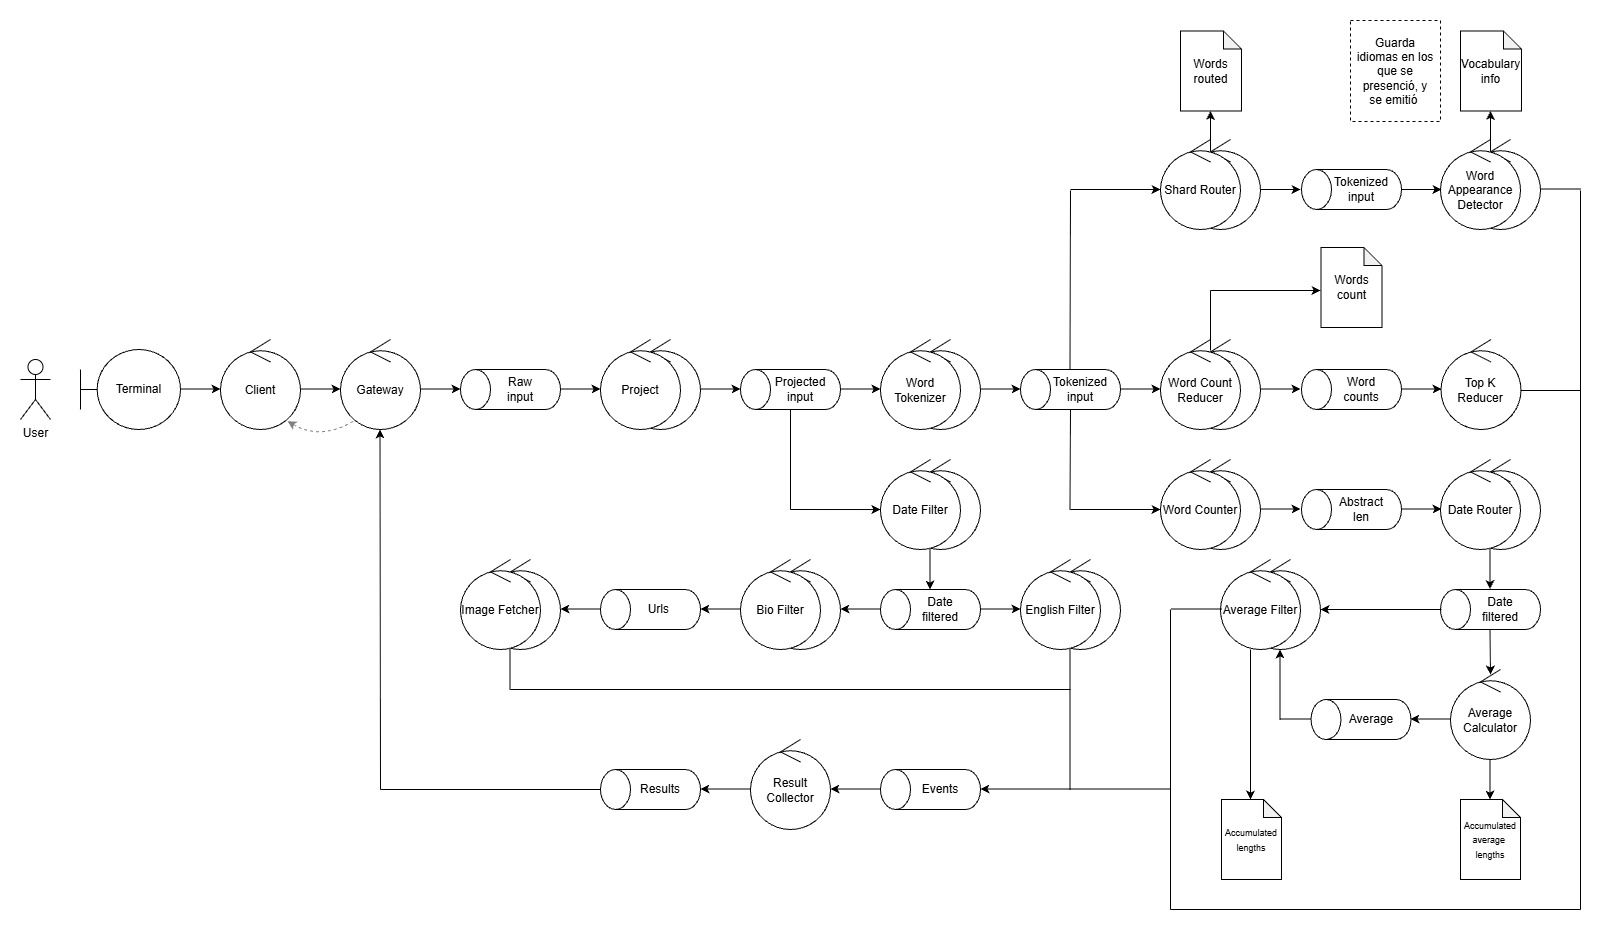
\includegraphics[width=\textwidth,height=0.82\textheight,keepaspectratio]{img/diagrama_de_robustez.jpg}
    \caption{Diagrama de robustez del sistema planteado}
    \label{fig:result-collector}
\end{figure}

El usuario inicia la ejecución desde \texttt{Terminal}, que se la entrega a  \texttt{Client}.  \texttt{Client} envía los artículos a  \texttt{Gateway}, que los publica en  \texttt{Raw input} identificados por cliente.  \texttt{Project} consume desde ahí, descarta las columnas que ninguna consulta necesita y publica en  \texttt{Projected input}. En ese momento, el flujo se divide dependiendo de la query: las primeras dos consultas partiendo de  \texttt{DateFilter}, y las últimas tres partiendo de  \texttt{WordTokenizer}.

Para las queries 1 y 2,  \texttt{Date Filter} descarta los artículos posteriores a 2020 y publica el resto en  \texttt{Date filtered}.  \texttt{EnglishFilter} consume de ese exchange, se queda con los artículos en inglés y envía sus resultados parciales a  \texttt{Events}.  \texttt{BioFilter} también consume de ahí, retiene los artículos que tienen una sección de biografía, y luego se descargan las imágenes de estos mediante  \texttt{ImageFetcher}, para luego enviar los resultados hacia  \texttt{Events}.

Para la query 3,  \texttt{WordTokenizer} publica las palabras únicas de cada abstract en  \texttt{Tokenized input}.  \texttt{ShardRouter} las agrupa en lotes por partición hasheandolas, registra el ruteo en el archivo  \texttt{Words routed} y las entrega a las instancias de  \texttt{WordAppearenceDetector}. Cada instancia conserva en el archivo  \texttt{Vocabulary info} los idiomas en que apareció cada palabra y cuáles ya emitió. Cuando una palabra aparece en inglés y en francés, la envía como resultado parcial a  \texttt{Events}. 

Para la query 4,  \texttt{WordCountReducer} consume  \texttt{Tokenized input} y acumula las unidades por palabra y partición. Vuelca a disco en el archivo  \texttt{Words count} el vocabulario para no saturar la memoria. Al finalizar, publica su top 20 local en  \texttt{Word counts}.  \texttt{TopKReducer} combina los tops de todas las particiones y envía el top 20 global a  \texttt{Events}.

Para la query 5,   \texttt{WordCounter} consume  \texttt{Tokenized input}, calcula la cantidad de palabras de cada abstract y publica en  \texttt{Abstract len}.  \texttt{DateRouter} lee esa cola y separa los registros por fecha. Los de 2020 o anteriores van a  \texttt{AverageCalculator}, que los acumula en el archivo  \texttt{Accumulated average lengths} y finalmente publica el promedio en la cola  \texttt{Average}. Los de 2021 en adelante van directamente a  \texttt{AverageFilter}, que los guarda en el archivo  \texttt{Accumulated lengths} hasta recibir el promedio desde  \texttt{Average}. Con el promedio definitivo, envía a  \texttt{Events} únicamente los artículos que lo superan.

Todas las consultas terminan pasando sus resultados a  \texttt{Events}, de donde consume  \texttt{ResultCollector}, que lleva la cuenta de los FIN por cliente. Cuando terminaron las cinco consultas, notifica el fin de la ejecución. Los resultados se publican en  \texttt{Results} y de allí llegan finalmente al  \texttt{Gateway}.


\subsection{Despliegue}
\label{subsec:despliegue}

Cada host del servicio ejecuta un motor Docker y aloja los contenedores
correspondientes a sus responsabilidades. La figura~\ref{fig:despliegue}
representa una distribución ilustrativa: los hosts A y B muestran cómo repartir
el trabajo entre computadoras, sin fijar una cantidad mínima ni máxima de
equipos. Las cajas de ingesta y workers agrupan procesos asignados a cada host;
no representan un único contenedor. Estos procesos pueden repartirse entre
varios contenedores o agruparse en uno, según la configuración de despliegue.
Un rol lógico del DAG tampoco exige un proceso ni una máquina exclusivos.

\paragraph{Distribución de responsabilidades.}
Los clientes conservan el dataset de entrada y envían registros incrementalmente
a \texttt{Gateway}, sin ejecutar las consultas ni conocer la topología de
RabbitMQ. Cada cliente tiene configurada la dirección del \texttt{Gateway}
con el que se comunica; varios clientes pueden utilizar la misma instancia.
Mostrar varios gateways ilustra una opción de escalado, sin incorporar un
router ni un balanceador adicional.

En el ejemplo, cada host de borde aloja un contenedor \texttt{Gateway} y otro
\texttt{ResultCollector}. El primero administra la sesión TCP y la admisión; el
segundo reúne los resultados de las consultas y sus cierres por ejecución.
Su ubicación conjunta es ilustrativa: pueden ejecutarse en hosts diferentes,
ya que se comunican mediante RabbitMQ. Cada ejecución identifica el Gateway
que conserva su conexión TCP y al que deben encaminarse los resultados.
El despliegue base no asigna archivos locales a \texttt{ResultCollector}:
reenvía lotes acotados y mantiene el seguimiento de entrega y finalización.

El host de mensajería aloja un contenedor RabbitMQ con los exchanges y colas
del middleware. Los hosts de cómputo alojan contenedores de ingesta y workers de
consultas, con archivos temporales en su propio disco. La tabla siguiente
relaciona estos grupos con los nombres de la propuesta actual.

\begin{center}
\small
\renewcommand{\arraystretch}{1.18}
\begin{tabular}{|p{0.20\textwidth}|p{0.70\textwidth}|}
\hline
\textbf{Grupo} & \textbf{Roles del DAG y ubicación} \\
\hline
Ingesta & \texttt{Project}: validación y proyección de los campos necesarios,
en hosts de cómputo. \\
\hline
Workers Q1/Q2 & \texttt{Date Filter}, \texttt{EnglishFilter},
\texttt{BioFilter} e \texttt{ImageFetcher}, en hosts de cómputo. \\
\hline
Workers Q3 & \texttt{WordTokenizer}, \texttt{Shard Router} y
\texttt{WordAppearenceDetector}: presencia de palabras por idioma. \\
\hline
Workers Q4 & \texttt{WordTokenizer}, \texttt{WordCountReducer} y
\texttt{TopKReducer}: conteos por palabra y top 20 por ejecución. \\
\hline
Workers Q5 & \texttt{WordTokenizer}, \texttt{Word Counter},
\texttt{Date Router}, \texttt{Average Calculator} y \texttt{Average Filter}:
conteos por abstract, promedio histórico y evaluación de candidatos. \\
\hline
Borde & \texttt{Gateway} y \texttt{ResultCollector}: entrada y salida TCP,
sesión y entrega de resultados. \\
\hline
\end{tabular}
\end{center}

\begin{figure}[p]
    \centering
    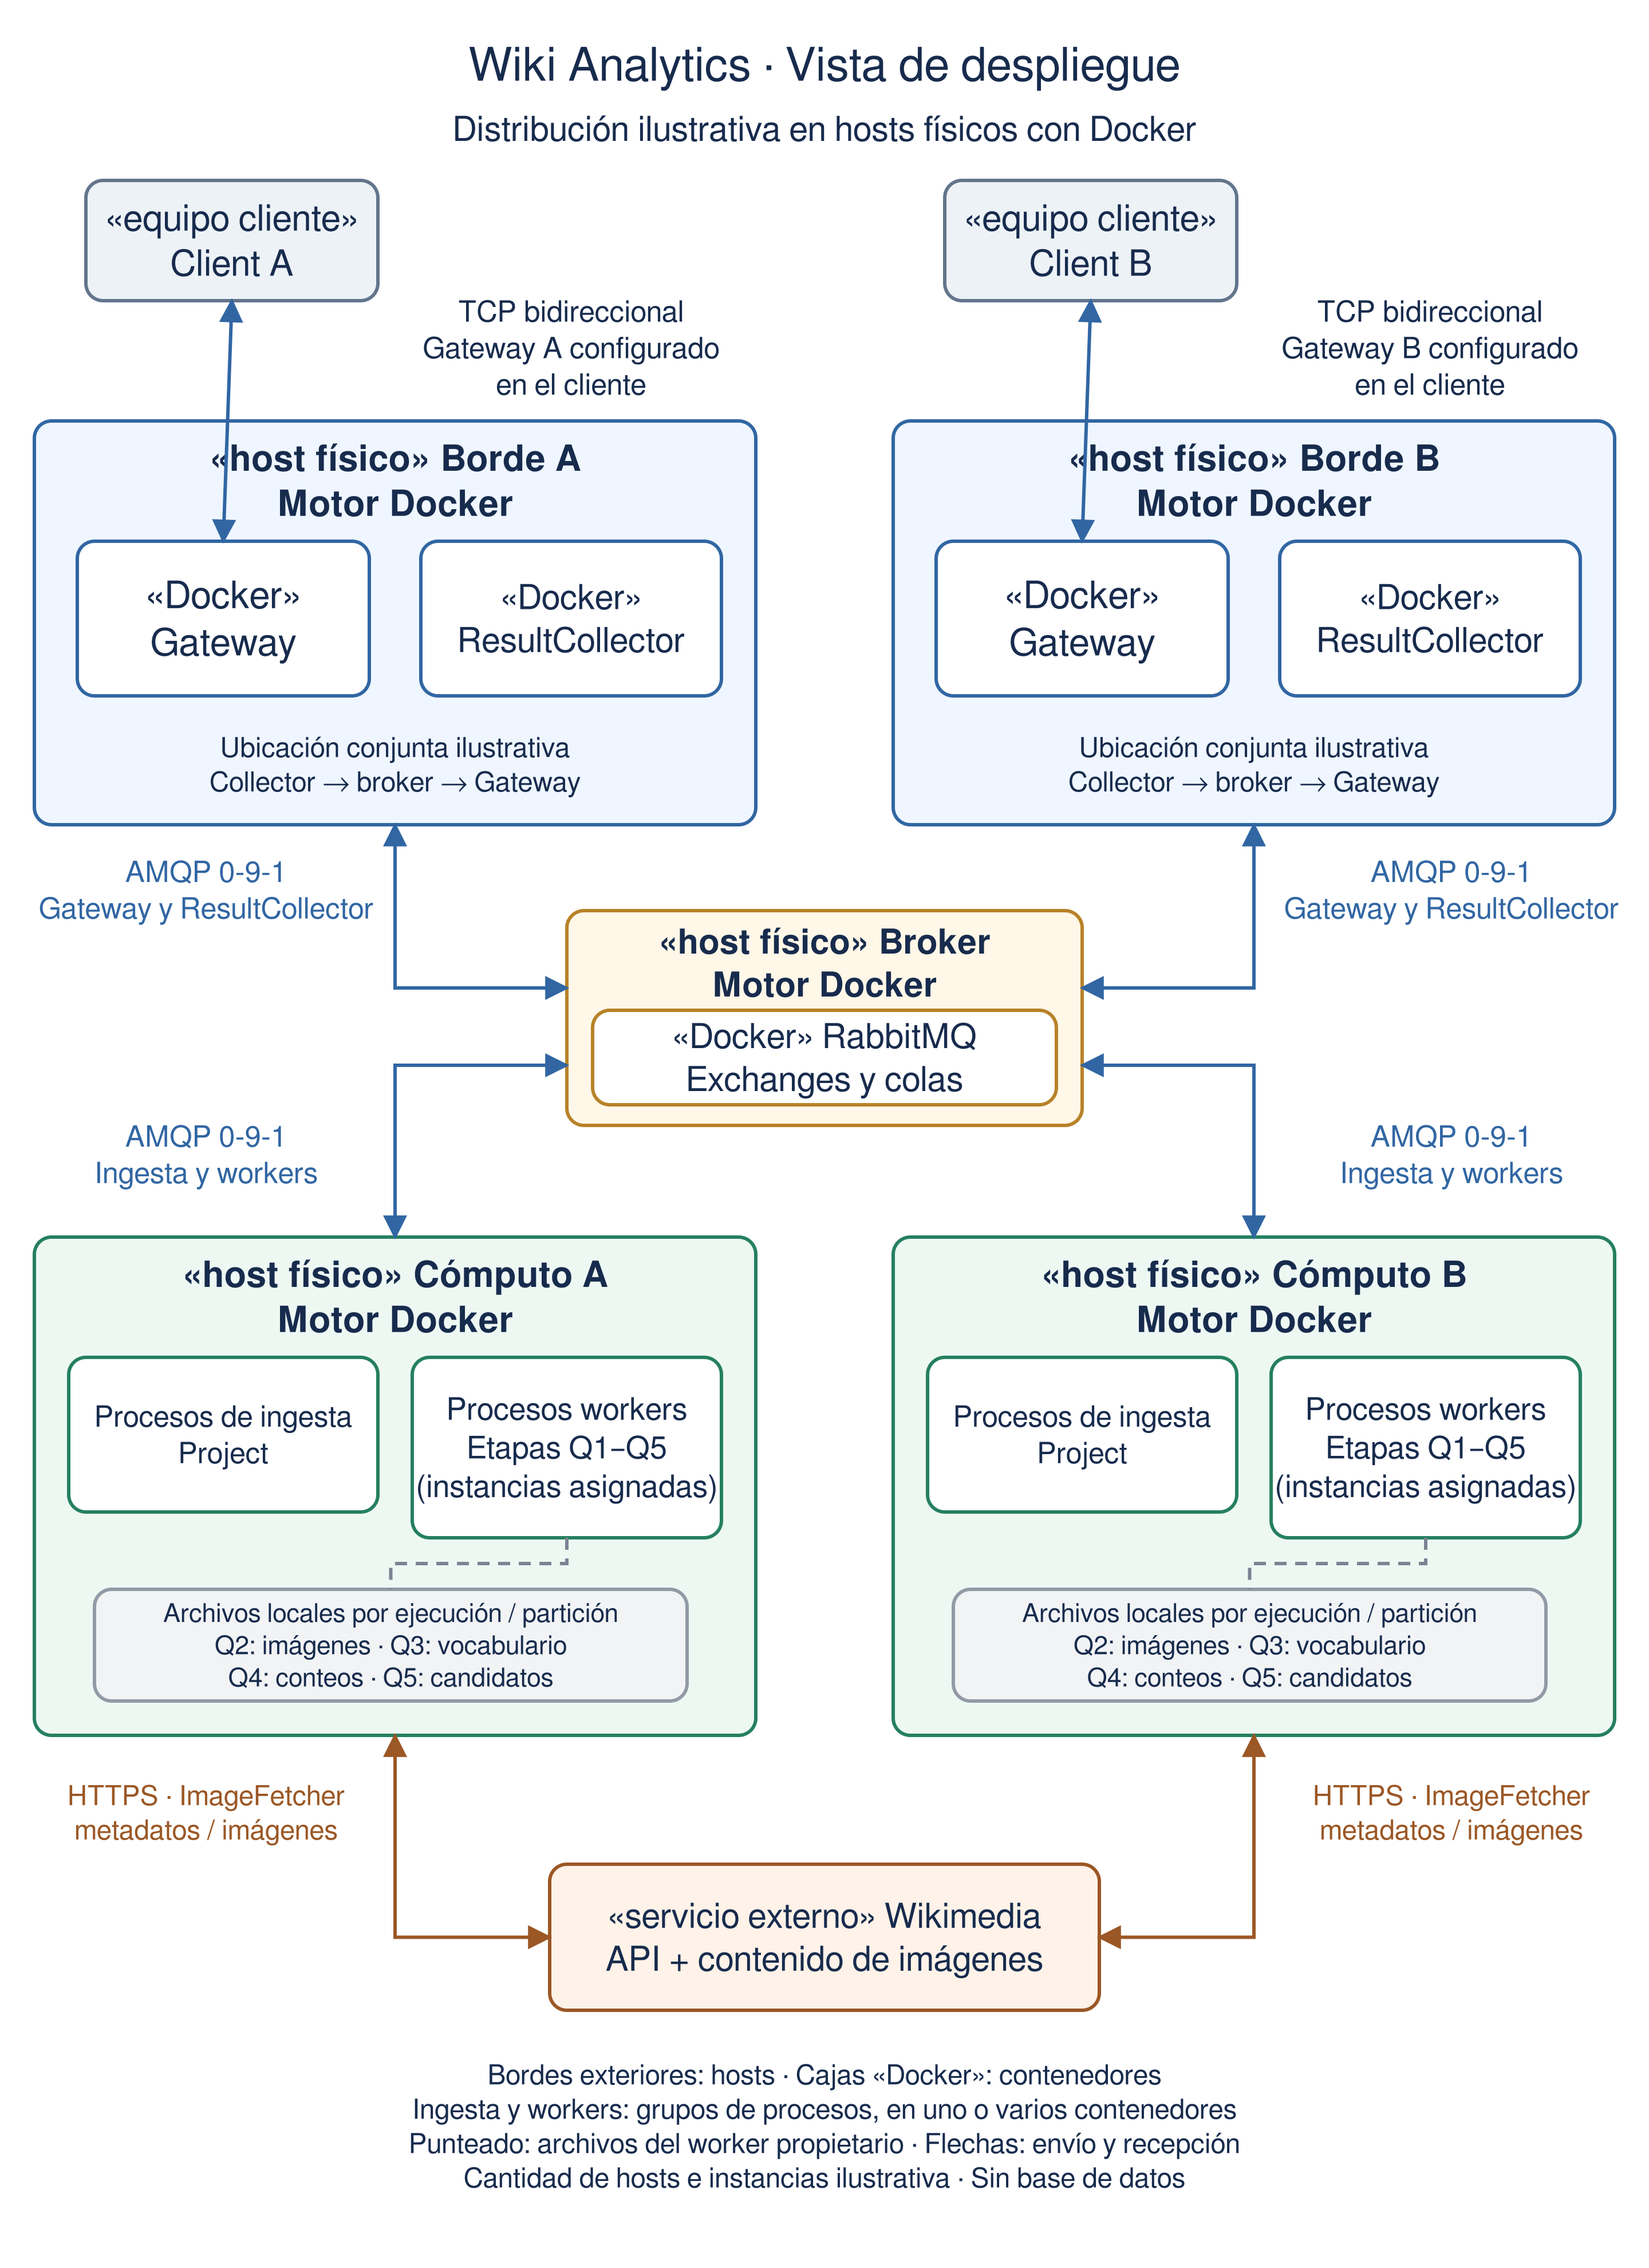
\includegraphics[width=\textwidth,height=0.82\textheight,keepaspectratio]{img/diagrama_de_despliegue.png}
    \caption{Despliegue ilustrativo del DAG en hosts físicos con contenedores
    Docker. Las cajas de ingesta y workers agrupan procesos, cuya distribución
    entre contenedores es configurable. Los enlaces AMQP conectan las instancias
    con el broker; HTTPS corresponde únicamente a ImageFetcher.}
    \label{fig:despliegue}
\end{figure}

Tanto Q4 como Q5 excluyen
stopwords y cuentan cada palabra una sola vez por abstract, conforme a la
decisión actual del equipo (el notebook de referencia no excluye palabras repetidas en Q5).

\paragraph{Enlaces de comunicación.}
El enlace \texttt{Client}--\texttt{Gateway} utiliza TCP bidireccional con
mensajes delimitados por longitud para transmitir artículos, resultados y
fragmentos de imágenes. El cliente debe recibir resultados mientras envía
entrada. Los contenedores del servicio intercambian datos y control mediante
AMQP 0-9-1 sobre RabbitMQ, incluido el envío de \texttt{ResultCollector} a
\texttt{Gateway}, aunque ambos estén en el mismo host. Los exchanges
\texttt{topic} enrutan hacia etapas y particiones; la difusión del umbral de Q5
debe alcanzar a cada destinatario mediante colas identificadas.

Sólo los contenedores que alojan \texttt{ImageFetcher} necesitan el enlace
HTTPS externo para resolver metadatos mediante la API de Wikimedia y obtener
los bytes desde la URL de contenido correspondiente. Las imágenes se entregan
por el circuito de resultados hasta \texttt{Gateway}. Las flechas entre hosts
resumen estas conexiones de los contenedores; no agregan comunicación directa
entre etapas que evite el middleware.

\paragraph{Asignación de trabajo y almacenamiento local.}
La configuración de despliegue asigna las particiones a instancias de workers
alojadas en contenedores. Esa asignación permanece fija durante cada ejecución;
un worker puede atender varias particiones. El criterio de particionado y el
aislamiento del estado se describen en la
sección~\ref{subsec:particionado-aislamiento}.

Los archivos temporales de Q2--Q5 residen en el disco del host de cómputo,
mediante montajes locales accesibles al worker propietario. No se introduce
una base de datos ni almacenamiento compartido entre hosts. El despliegue debe
proveer memoria y disco acordes con las cuotas de las instancias alojadas;
la responsabilidad sobre esos archivos, su ciclo de vida y el control de
recursos se detallan en la sección~\ref{subsec:estado-recursos}.

\paragraph{Escalabilidad y operación.}
Un único Gateway puede atender múltiples clientes concurrentes. Para ampliar
la capacidad de entrada y salida se pueden agregar gateways y propietarios de
ejecuciones, eventualmente en nuevos hosts de borde. Los clientes se asignan
por configuración a esas instancias; no se promete selección transparente ni
migración de sesiones entre gateways. Para procesar mayor volumen por cliente se agregan hosts de
cómputo y se distribuyen las particiones antes de las nuevas ejecuciones.
Los contenedores conservan el mismo DAG y contrato semántico. Persisten límites
en el broker, la salida de cada ejecución por su \texttt{Gateway} y
\texttt{ResultCollector}, y las particiones con palabras muy frecuentes.
Los recursos se dimensionan según la carga; no se promete crecimiento lineal
ilimitado.

Ante SIGTERM se detiene la admisión y se coordina el drenaje de las ejecuciones
activas. Los procesos Go deben recibir la señal; el plazo de parada de Docker
debe permitir drenar o notificar una cancelación explícita. Se cierran archivos
y conexiones después de confirmar las operaciones pendientes, y RabbitMQ se
detiene al final del apagado coordinado. No se anuncia éxito al cancelar.

Una caída abrupta de un propietario o la pérdida de sus archivos aborta las
ejecuciones afectadas. Una caída de \texttt{Gateway} invalida sus sesiones;
la del broker invalida las ejecuciones dependientes. El cliente reinicia con
una identidad nueva y retransmite todo el input, sin acumular resultados del
intento anterior. Reiniciar un contenedor no recupera sus ejecuciones.
El broker único por instalación no implica alta disponibilidad.

